\documentclass{article}
\usepackage{tikz}
\usepackage{caption}
\usepackage{subcaption}
\usepackage{float}


\title{Intro to Linguistics - HW2 - Syntax}
\author{Andrew McIsaac}

\begin{document}
\maketitle

\begin{enumerate}
	\item{Analyze these sentences (or phrases)}
		\begin{enumerate}
			\item{The monkey ate a banana and a big melon.}
				\begin{figure}[H]
					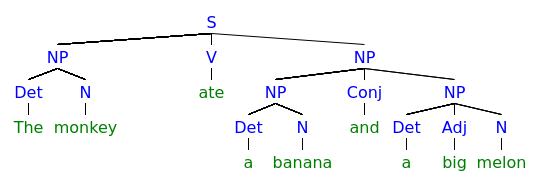
\includegraphics[width=\linewidth]{1a.png}
					\label{fig:1a}
				\end{figure}
			\item{The small monkey gave me a banana.}
				\begin{figure}[H]
					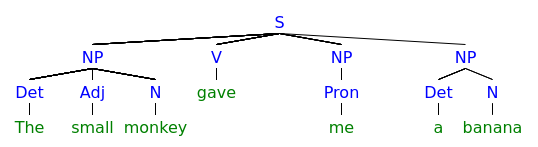
\includegraphics[width=\linewidth]{1b.png}
					\label{fig:1b}
				\end{figure}
			\item{The monkey gave a banana to me.}
				\begin{figure}[H]
					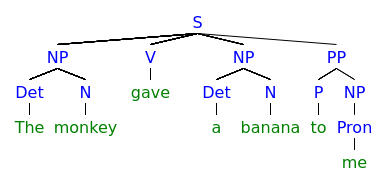
\includegraphics[width=\linewidth]{1c.png}
					\label{fig:1c}
				\end{figure}
			\item{George saw the big dog of my friend.}
				\begin{figure}[H]
					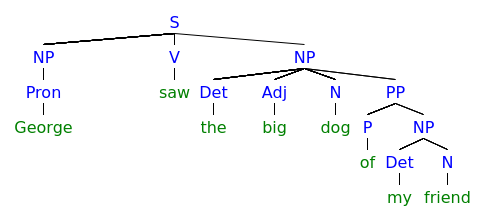
\includegraphics[width=\linewidth]{1d.png}
					\label{fig:1d}
				\end{figure}
			\item{The shop is at the corner of the street.}
				\begin{figure}[H]
					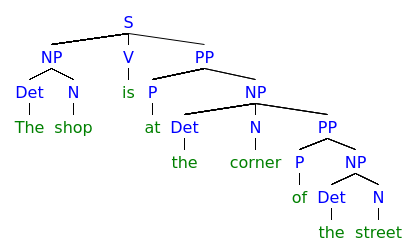
\includegraphics[width=\linewidth]{1e.png}
					\label{fig:1e}
				\end{figure}
			\item{The parents of the groom and the bride.}
				\begin{figure}[H]
					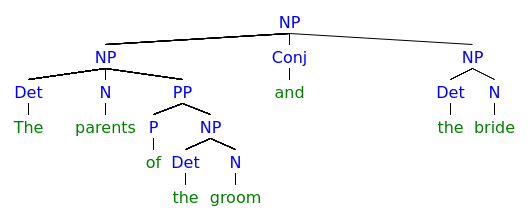
\includegraphics[width=\linewidth]{1fi.png}
					\label{fig:1fi}
				\end{figure}
				\begin{figure}[H]
					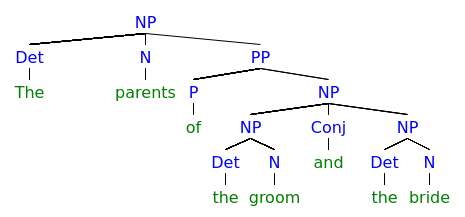
\includegraphics[width=\linewidth]{1fii.png}
					\label{fig:1fii}
				\end{figure}
			\item{His son sings and her daughter plays the piano.}
				\begin{figure}[H]
					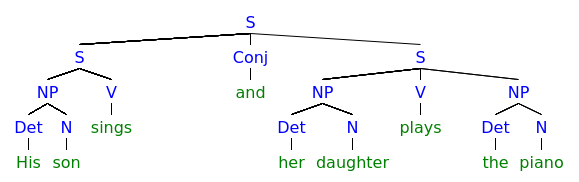
\includegraphics[width=\linewidth]{1g.png}
					\label{fig:1g}
				\end{figure}
		\end{enumerate}

	\item{Find:}
		\begin{enumerate}
			\item{Two sentences that are correct according to both this grammar
					and grammar of Standard English  (GSE). Draw the
					corresponding syntactic trees.}
						\begin{figure}[H]
							\begin{subfigure}[b]{0.3\linewidth}
								\centering
								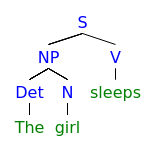
\includegraphics[width=\linewidth]{2ai.png}
								\caption{The girl sleeps.}
								\label{fig:2ai}
							\end{subfigure}
							\hfill
							\begin{subfigure}[b]{0.6\linewidth}
								\centering
								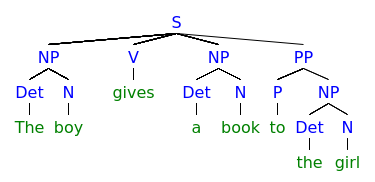
\includegraphics[width=\linewidth]{2aii.png}
								\caption{The boy gives a book to the girl.}
								\label{fig:2aii}
							\end{subfigure}
							\label{fig:2a}
						\end{figure}
			\item{A sentence that is correct according to this grammar, but
				incorrect according to GSE. Where is the problem?}

				*``A girl gives a boy book.''

				A determiner is required before `book', but is optional in this
				grammar.
			\item{A sentence that is incorrect according to this grammar, but
				correct according to GSE. Where is the problem?}
			
				``The boy sees the interesting small girl.''

				Two adjectives are not allowed to modify a single noun in this
				grammar, but it is possible in GSE.
		\end{enumerate}


\end{enumerate}

\end{document}
